\documentclass[12pt,twosided,titlepage]{article}
\usepackage{fancyhdr}
\usepackage{graphicx}
\usepackage{psfrag}
\usepackage{cancel}
\usepackage{fullpage}
\usepackage{bm}
%\usepackage{palatino} % this is the recommended font
\usepackage{amsthm}
\usepackage{amsmath,epsfig,latexsym,amssymb,rotating}
\usepackage[usenames,dvipsnames]{color}
\usepackage{ulem}
\usepackage{soul}
\usepackage{listings}
\usepackage{xcolor}
%\usepackage{geometry}
%\geometry{left=2.5cm,right=2.5cm,top=2.5cm,bottom=2.5cm}
%---Adjust row spacing of items---
\usepackage{paralist}
\let\itemize\compactitem
%\let\enditemize\endcompactitem
%---------------------------------
%\usepackage{ntheorem}
% Define some useful tools for these notes
\newenvironment{thinlist}[1][\labelitemi]{\begin{list}{#1}{\topsep=\smallskipamount \parsep=\smallskipamount \itemsep=\smallskipamount}}{\end{list}}
\renewcommand{\baselinestretch}{1.2}
\numberwithin{equation}{section}

\DeclareMathOperator*{\rank}{rank}
\DeclareMathOperator*{\diag}{diag}
\DeclareMathOperator*{\argmin}{argmin}
\DeclareMathOperator*{\Argmin}{Argmin}

\lstset{
numbers=left,
    numberstyle= \tiny,
    keywordstyle= \color{ blue!70},
    commentstyle= \color{red!50!green!50!blue!50},
    frame=shadowbox, % ��ӰЧ��
    rulesepcolor= \color{ red!20!green!20!blue!20} ,
    escapeinside=``, % Ӣ�ķֺ��п�д������
    xleftmargin=2em,xrightmargin=2em, aboveskip=1em,
    framexleftmargin=2em
}

\begin{document}

\newtheorem{thm}{Theorem}[section]
\newtheorem{prop}{Proposition}[section]
\newtheorem{lemma}{Lemma}[section]
\newtheorem{cor}{Corollary}[section]
\newtheorem{mydef}{Definition}[section]
\newtheorem{example}{Example}[section]

\def \bC {\mathbb C}
\def \bR {\mathbb R}
\def \bN {\mathbb N}
\def \bS {\mathbb S}
\def \bZ {\mathbb Z}
\def \bRn {\bR^n}
\def \bRm {\bR^m}
\def \bRK {\bR^K}
\def \bRKp {\bR^{K+1}}
\def \bRT {\bR^T}
\def \bRmn {\bR^{m\times n}}
\def \bRnm {\bR^{n\times m}}
\def \bRnn {\bR^{n\times n}}
\def \bRmm {\bR^{m\times m}}
\def \bSpn {\bS_+^{n}}
\def \bSppn {\bS_{++}^{n}}

\def \tr {\mathrm{tr}}
\def \var {\mathrm{var}}
\def \cov {\mathrm{cov}}
\def \sgn {\mathrm{sgn}}
\def \range {\mathrm{range}}
\def \prox {\mathrm{prox}}
\def \diag {\mathrm{diag}}

\def \bmA {\bm A}
\def \bmB {\bm B}
\def \bmC {\bm C}
\def \bmD {\bm D}
\def \bmH {\bm H}
\def \bmI {\bm I}
\def \bmK {\bm K}
\def \bmL {\bm L}
\def \bmP {\bm P}
\def \bmQ {\bm Q}
\def \bmR {\bm R}
\def \bmS {\bm S}
\def \bmT {\bm T}
\def \bmU {\bm U}
\def \bmV {\bm V}
\def \bmW {\bm W}
\def \bmX {\bm X}
\def \bmY {\bm Y}
\def \bmZ {\bm Z}
\def \bmalpha {\bm\alpha}
\def \bmsigma {\bm\sigma}
\def \bmbeta {\bm\beta}
\def \bmepsi {\bm\epsilon}
\def \bmtheta {\bm\theta}
\def \bmeta {\bm\eta}
\def \bmLambda {\bm\Lambda}
\def \bmSigma {\bm\Sigma}
\def \bma {\bm a}
\def \bmb {\bm b}
\def \bmc {\bm c}
\def \bmd {\bm d}
\def \bme {\bm e}
\def \bmh {\bm h}
\def \bml {\bm l}
\def \bmp {\bm p}
\def \bmq {\bm q}
\def \bmr {\bm r}
\def \bms {\bm s}
\def \bmu {\bm u}
\def \bmv {\bm v}
\def \bmw {\bm w}
\def \bmx {\bm x}
\def \bmy {\bm y}
\def \bmz {\bm z}

\def \tbmw {\tilde{\bm w}}
\def \tbmx {\tilde{\bm x}}
\def \tbeta {\tilde{\beta}}
\def \tb {\tilde{b}}
\def \tsigma {\tilde{\sigma}}

\def \mcH {\mathcal{H}}
\def \mcI {\mathcal{I}}
\def \mcK {\mathcal{K}}
\def \mcL {\mathcal{L}}
\def \mcN {\mathcal{N}}

\def \FixT {\text{Fix}{(T)}}

\newpage
\begin{center}
\begin{tabular}{|c c c|}
\hline
%& &\\
& Mathematical Modeling & \\
& \textbf{Lecture 1. One Variable Optimization}  &  \\
%& {\small STAT 440 / 840, CM 461} &  \\
& {\small Yizun Lin} &  \\
& Department of Mathematics, Jinan University & \\
& \today & \\
\hline
\end{tabular}
\end{center}
\vspace{1em}

\section{The Five-step Method}
\begin{example}\label{PigExamp1}
A pig weighing 200 pounds gains 5 pounds per day and costs 45 cents a day to keep. The market price for pigs is 65 cents per pound, but is falling 1 cent per day. When should the pig be sold?
\end{example}

\hspace{-1.5em}The mathematical modeling approach to problem solving consists of five steps:
\begin{itemize}
\item[1.] Ask the question.
\item[2.] Select the modeling approach.
\item[3.] Formulate the model.
\item[4.] Solve the model.
\item[5.] Answer the question.
\end{itemize}

\vspace{1em}
\hspace{-1.5em}{\bf Step 1. Ask the question}

The question must be phrased in mathematical terms and there are three stages of step 1 as follows.

\vspace{0.5em}
\begin{tabular}{ll}
{\bf Variables:}&$t$ = time (days)\\
&$w$ = weight of pig (lbs)\\
&$p$ = price for pigs (\$/lb)\\
&$C$ = cost of keeping pig $t$ days (\$)\\
&$R$ = revenue obtained by selling pig (\$)\\
&$P$ = profit from sale of pig (\$)\\\vspace{-0.6em}
&\\
{\bf Assumptions:}&$w=200+5t$\\
&$p=0.65-0.01t$\\
&$C=0.45t$\\
&$R=p\cdot w$\\
&$P=R-C$\\
&$t\geq0$\\\vspace{-0.6em}
&\\
{\bf Objective:}&Maximize $P$
\end{tabular}
\newpage

\hspace{-1.5em}{\bf Step 2. Select the modeling approach}
\begin{itemize}
\item Many types of problems can be stated in a standard form for which an effective general solution procedure exists.
\item Our example problem can be modeled as a one-variable optimization problem (or maximum-minimum problem).
\end{itemize}

We are given a real-valued function $y=f(x)$ defined on a subset $S$ of the real line. There is a theorem that states that if $f$ attains its maximum or minimum at an interior point $x\in S$, then $f'(x)=0$, assuming that $f$ is differentiable at $x$. This allows us to rule out any interior point $x\in S$ at which $f'(x)=0$ as a candidate for max-min. This procedure works well as long as there are not too many exceptional points.

\vspace{1em}
\hspace{-1.5em}{\bf Step 3. Formulate the model}

Take the question exhibited in step 1 and reformulate it in the standard form selected in step 2.

For Example \ref{PigExamp1}, we have
\begin{align*}
P&=R-C\\
&=p\cdot w-0.45t\\
&=(0.65-0.01t)(200+5t)-0.45t
\end{align*}
Let $y=P$ be the quantity we wish to maximize. Then our problem now is to maximize and $x=t$ the independent variable. Our problem now is to maximize
\begin{align}
\notag y&=f(x)\\
\notag &=(0.65-0.01x)(200+5x)-0.45x\\
\label{eq:PigExamp1}&=-0.05x^2+0.8x+130
\end{align}
over the set $S=\{x:x\geq0\}$.

\vspace{1em}
\hspace{-1.5em}{\bf Step 4. Solve the model}

In Example \ref{PigExamp1}, we want to find the maximum of the function $y=f(x)$ defined by Eq. \eqref{eq:PigExamp1} over the set $x\geq0$. Figure \ref{fig1:PigExamp} shows a graph of the function $f(x)$. Since $f$ is quadratic in $x$, the graph is a parabola. We compute that
$$
f'(x)=-\frac{1}{10}(x-8),
$$
so that $f'(x)=0$ at the point $x=8$. Since $f$ is increasing on the interval $(-\infty,8)$ and decreasing on $(8,+\infty)$, the point $x=8$ is the global maximum. At this point we have $y=f(8)=133.2$. Since the point $(x,y)=(8,133.2)$ is the global maximum of $f$ over the entire real line, it is also the maximum over the set $x\geq0$.

\begin{figure}[htbp]
\centering
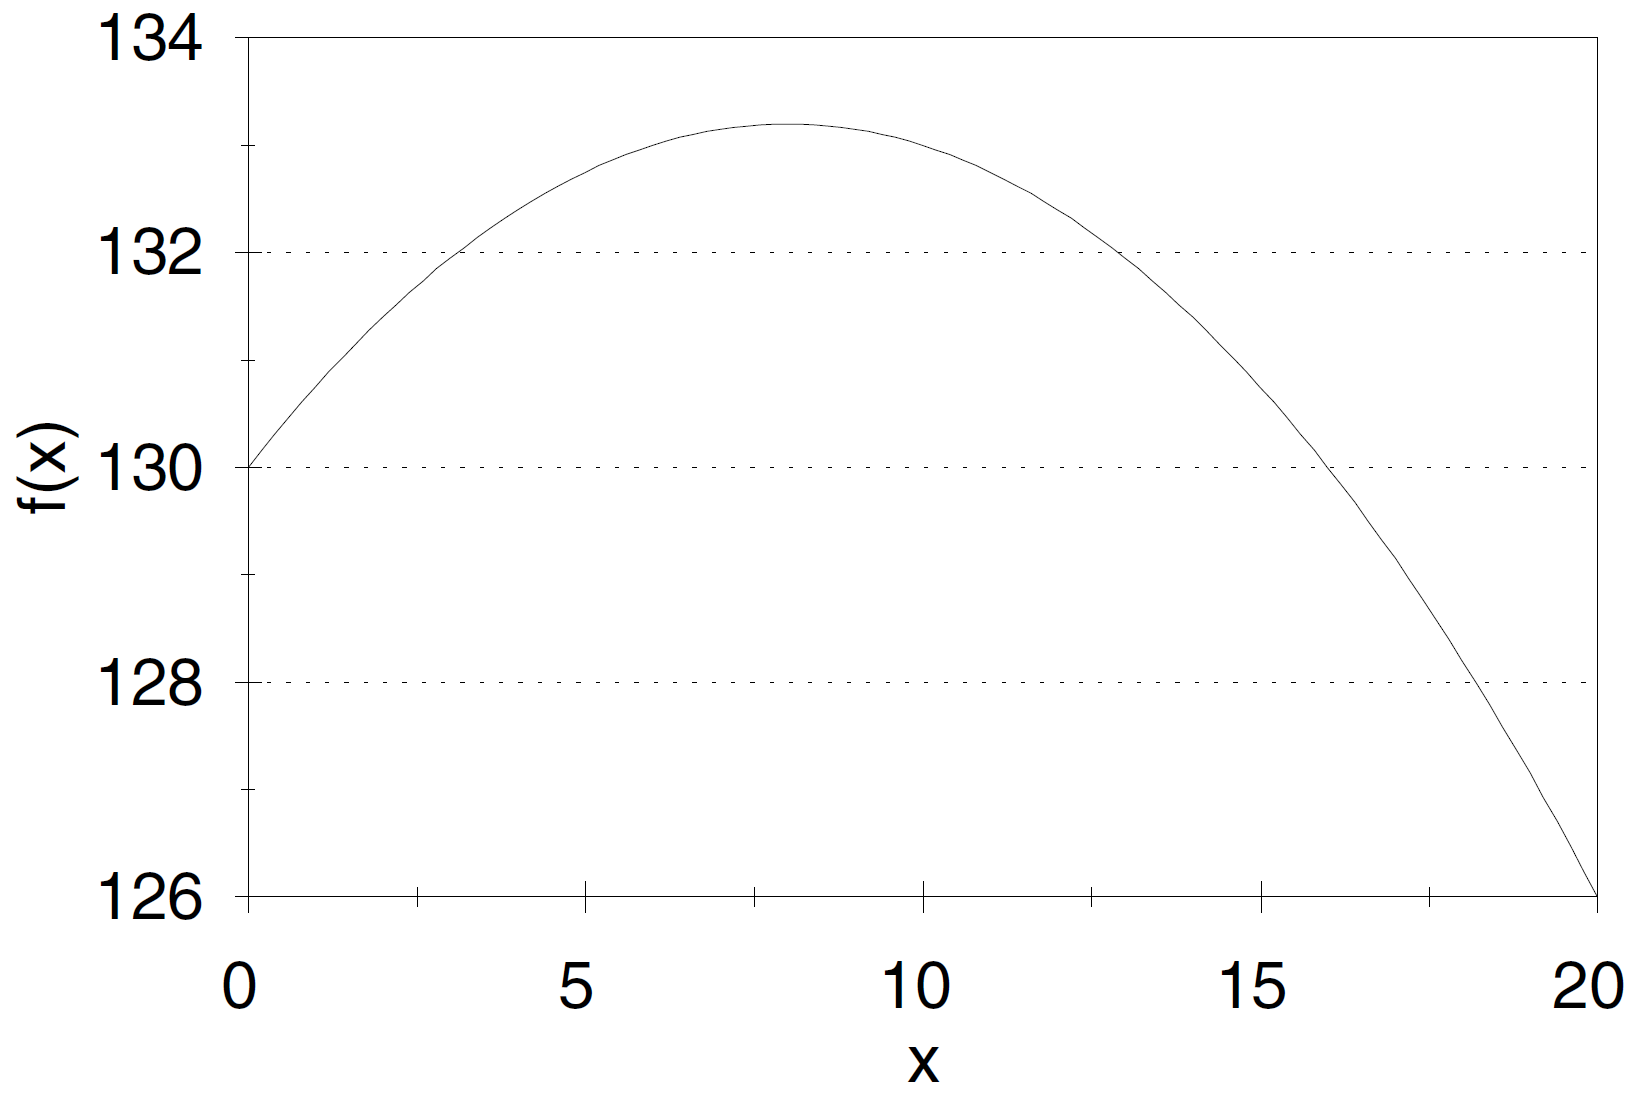
\includegraphics[scale=0.2]{figs/PigExampFig1.png}
\caption{Graph of net profit $f(x)=-0.05x^2+0.8x+130$ versus time to sell $x$ for the pig problem.}
\label{fig1:PigExamp}
\end{figure}

\vspace{1em}
\hspace{-1.5em}{\bf Step 5. Answer the question}

In Example \ref{PigExamp1}, we need to answer when to sell the pig in order to maximize profit. The answer obtained by our mathematical
model is to sell the pig after 8 days, thus obtaining a net profit of \$133.2. This answer is valid as long as the assumptions made in step 1 remain valid.

\vspace{1em}
\hspace{-1.5em}{\bf\large Conclusion:}

\vspace{1em}
\hspace{-1.5em}{\bf Step 1. Ask the question.}
\begin{itemize}
\item Make a list of all the variables in the problem, including appropriate units.
\item Be careful not to confuse variables and constants.
\item State any assumptions you are making about these variables, including equations and inequalities.
\item Check units to make sure that your assumptions make sense.
\item State the objective of the problem in precise mathematical terms.
\end{itemize}

\vspace{1em}
\hspace{-1.5em}{\bf Step 2. Select the modeling approach.}
\begin{itemize}
\item Choose a general solution procedure to be followed in solving this problem.
\item Generally speaking, success in this step requires experience, skill, and familiarity with the relevant literature.
\item In this book we will usually specify the modeling approach to be used.
\end{itemize}

\vspace{1em}
\hspace{-1.5em}{\bf Step 3. Formulate the model.}
\begin{itemize}
\item Restate the question posed in step 1 in the terms of the modeling approach
specified in step 2.
\item You may need to relabel some of the variables specified in step 1 in order to agree with the notation used in step 2.
\item Note any additional assumptions made in order to fit the problem described in step 1 into the mathematical structure specified in step 2.
\end{itemize}

\vspace{1em}
\hspace{-1.5em}{\bf Step 4. Solve the model.}
\begin{itemize}
\item Apply the general solution procedure specified in step 2 to the specific problem formulated in step 3.
\item Be careful in your mathematics. Check your work for math errors. Does
your answer make sense?
\item Use appropriate technology. Computer algebra systems, graphics, and numerical software will increase the range of problems within your grasp, and they also help reduce math errors.
\end{itemize}

\vspace{1em}
\hspace{-1.5em}{\bf Step 5. Answer the question.}
\begin{itemize}
\item Rephrase the results of step 4 in nontechnical terms.
\item Avoid mathematical symbols and jargon.
\item Anyone who can understand the statement of the question as it was presented to you should be able to understand your answer.
\end{itemize}

\section{Sensitivity Analysis}
The process of mathematical modeling begins by making some assumptions about the problem. We are rarely certain enough to expect all of these assumptions to be exactly valid. Therefore, we need to consider how sensitive our conclusions are to each of the assumptions we have made.

Look back on the pig problem. The following data are easy to measure and can be known with much more certainty:
\begin{itemize}
\item the current weight of the pig,
\item the current price for pigs,
\item the cost per day of keeping the pig.
\end{itemize}
However, the rate of growth of the pig is a bit less certain, and the rate at which the price is falling is even less certain.

Let $r$ denote the rate at which the price is falling. We assumed that $r=0.01$ dollars per day, but let us now suppose that the actual value of $r$ is different. By repeating the solution procedure for several different values of $r$, we can get an idea of the sensitivity of our answer to the value of $r$.

A more systematic method for measuring this sensitivity would be to treat $r$ as an unknown parameter, following the same steps as before. Writing $p=0.65-rt$, we can proceed as before to obtain
\begin{align*}
y&=f(x)\\
&=(0.65-rx)(200+5x)-0.45x\\
&=-5rx^2+(2.8-200r)x+130.
\end{align*}
Then we can compute
$$
f'(x)=-\frac{2}{5}(25rx+500r-7)
$$
so that $f'(x)=0$ at the point
\begin{equation}\label{eq:L1sensrx}
x=\frac{7}{25r}-20.
\end{equation}
The optimal time to sell is given by Eq. \eqref{eq:L1sensrx} as long as this expression is
positive, i.e., as long as $0<r\leq0.014$. For $r>0.014$, the vertex of the parabola $y=f(x)$ lies outside of the set $x\geq0$ over which we are maximizing. In this case the optimal time to sell is at $x=0$ since we have $f'(x)<0$ on the entire interval $[0,+\infty)$. See Figure \ref{fig4:PigExamp} for an illustration in the case $r=0.015$.
\begin{table}[htbp]
\centering
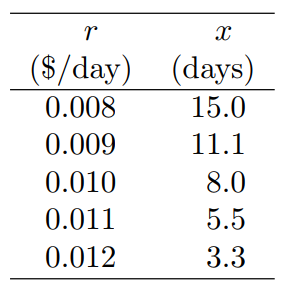
\includegraphics[scale=0.4]{figs/PigExampFig2.png}
\caption{Sensitivity of best time to sell $x$ to price falling rate $r$ for the pig problem.}
\label{fig2:PigExamp}
\end{table}

\begin{figure}[htbp]
\centering
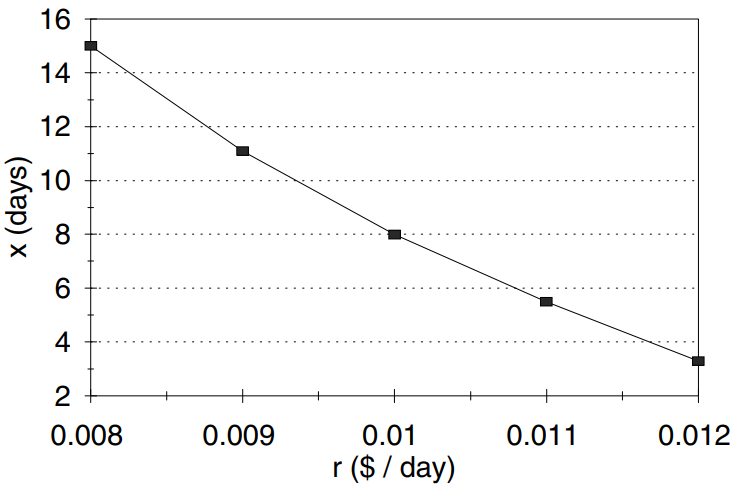
\includegraphics[scale=0.4]{figs/PigExampFig3.png}
\caption{Graph of best time to sell $x$ versus price falling rate $r$ for the pig problem.}
\label{fig3:PigExamp}
\end{figure}

\begin{figure}[htbp]
\centering
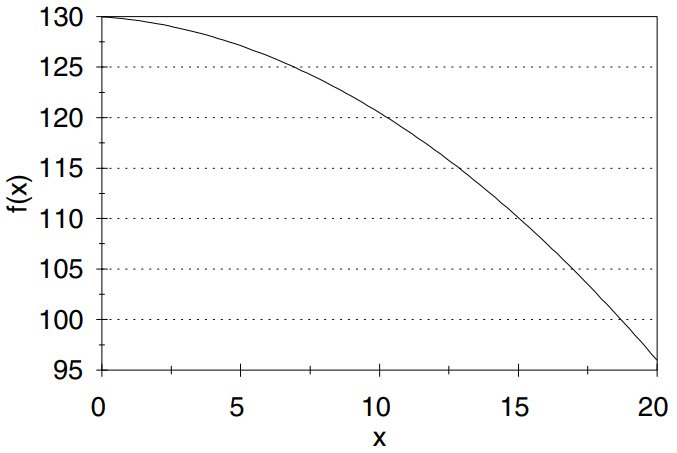
\includegraphics[scale=0.4]{figs/PigExampFig4.png}
\caption{Graph of net profit $f(x)=(0.65-0.015x)(200+5x)-0.45x$ versus time to sell $x$ for the pig problem in the case $r=0.015$.}
\label{fig4:PigExamp}
\end{figure}

We are also uncertain about the growth rate $g$ of the pig. We have assumed that $g=5$ lbs/day. More generally, we have that $w=200+gt$, which leads to the equation
\begin{align}
\notag f(x)&=(0.65-0.01x)(200+gx)-0.45x,\\
\label{eq:L1sensgfx}&=-0.01gx^2+(0.65g-2.45)x+130
\end{align}
so that
$$
f'(x)=-\frac{1}{100}(2gx-65g+245).
$$
Now $f'(x)=0$ at the point
\begin{equation}\label{eq:L1sensgx}
x=\frac{65}{2}-\frac{245}{2g}.
\end{equation}
The optimal time to sell is given by Eq. \eqref{eq:L1sensgx} so long as it represents a nonnegative value of $x$. Figure \ref{fig5:PigExamp} shows the relationship between the growth rate $g$ and the optimal time to sell.

\begin{figure}[htbp]
\centering
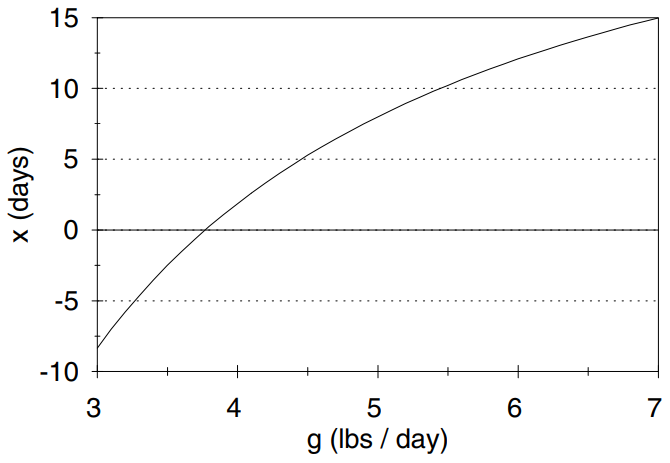
\includegraphics[scale=0.4]{figs/PigExampFig5.png}
\caption{Graph of best time to sell $x$ versus growth rate $g$ for the pig problem.}
\label{fig5:PigExamp}
\end{figure}

It is most natural and most useful to interpret sensitivity data in terms of relative change or percent change, rather than in absolute terms. If $x$ changes by an amount $\Delta x$, the relative change in $x$ is given by $\Delta x/x$. If $r$ changes
by $\Delta r$, resulting in the change $\Delta x$ in $x$, then the ratio between the relative changes is $\Delta x/x$ divided by $\Delta r/r$. Letting $\Delta r\to0$ and using the definition of the derivative, we obtain
$$
\frac{\Delta x/x}{\Delta r/r}\to\frac{dx}{dr}\cdot\frac{r}{x}
$$
We call this limiting quantity the sensitivity of $x$ to $r$, and we will denote it by $S(x,r)$. In the pig problem we have
$$
\frac{dx}{dr}=-\frac{7}{25r^2}=-2800
$$
at the point $r=0.01$ and $x=8$; thus
\begin{align*}
S(x,r)&=\frac{dx}{dr}\cdot\frac{r}{x}\\
&=(-2800)\times\frac{0.01}{8}\\
&=-\frac{7}{2}
\end{align*}
If $r$ goes up by $2\%$, then $x$ goes down by about $7\%$. Since
$$
\frac{dx}{dg}=\frac{245}{2g^2}=4.9
$$
at the point $g=5$ and $x=8$, we have
\begin{align*}
S(x,g)&=\frac{dx}{dg}\cdot\frac{g}{x}\\
&=4.9\times\frac{5}{8}\\
&=3.0625,
\end{align*}
so that a 1\% increase in the growth rate of the pig would cause us to wait about 3\% longer to sell the pig.

In order to compute the sensitivity $S(y,g)$, first substitute \eqref{eq:L1sensgx} into the objective function $y=f(x)$ from \eqref{eq:L1sensgfx} to obtain
\begin{align*}
y&=-0.01g\left(\frac{65}{2}-\frac{245}{2g}\right)^2+(0.65g-2.45)\left(\frac{65}{2}-\frac{245}{2g}\right)+130\\
&=-\frac{1}{200}(65g-245)\left(\frac{65}{2}-\frac{245}{2g}\right)+\frac{1}{100}(65g-245)\left(\frac{65}{2}-\frac{245}{2g}\right)+130\\
&=\frac{1}{200}(65g-245)\left(\frac{65}{2}-\frac{245}{2g}\right)+130\\
&=\frac{1}{400g}(65g-245)^2+130\\
&=\frac{150.0625}{g}+10.5625g+50.375.
\end{align*}
Then compute the derivative
$$
\frac{dy}{dg}=-\frac{150.0625}{g^2}+10.5625,
$$
and substitute $g=5$ to get $\frac{dy}{dg}=4.56$, which leads to
\begin{align*}
S(y,g)&=\frac{dy}{dg}\cdot\frac{g}{y}\\
&=4.56\times\frac{5}{133.2}\\
&=\frac{19}{111}\approx0.17.
\end{align*}
If the pig grows 10\% faster than expected, the expected net profit will be about 1.7\% larger.

It is usually not possible to compute sensitivity coefficients for each parameter in the model, nor is this particularly desirable. We need to select those parameters about which there is the most uncertainty and perform sensitivity analysis on them. In the pig problem, we are probably considerably more certain of the growth rate $g$ than of the price falling rate $r$. A 25\% error in $g$ would be quite surprising if we have observed the past history of growth in this pig. A 25\% error in our estimate of $r$ would not be at all surprising.

\vspace{2em}
\hspace{-1.5em}{\bf\color{red} Homework:}\\
Textbook, P16, Exercise 1(a)(b)(c) and 2.



\end{document}
